\documentclass[a4paper]{article}
\usepackage[utf8]{inputenc}
\usepackage[russian]{babel}
\usepackage{listings}
\usepackage[a4paper]{geometry}
\usepackage{indentfirst}
\usepackage{graphicx}
\usepackage{caption}
\usepackage{float}
\usepackage{amssymb}

\begin{document}

\title{Лабораторная работа 4 по курсу <<Нелинейная динамика и её приложения>>. \\Отчёт.}
\author{Владислав Соврасов\\ 381503м4}
\date{}
\maketitle

\section{Построение гистограммы распределения собственных чисел случайных матриц}
Рассмотрим симметричные матрицы \(A\in \mathbf{R}^{N\times N}\) такие, что \(A=A^T\) и
\begin{displaymath}
	a_{i,j} = \left\{
  \begin{array}{lr}
    2\mathcal{N}(0,1), i=j\\
		\mathcal{N}(0,1), i	\neq j
  \end{array}
\right.
\end{displaymath}
Известно, что такие матрицы (Gaussian Orthogonal Ensemble) имеют \(N\) действительных собственных чисел, которые
распределены по закону \(\rho(\lambda / \sqrt{N})=c \sqrt{4-\lambda^2/N}\), где
\(c\) --- нормировочная константа.

Для построения гистограммы распределения нормированных собственных чисел были
сгенерированы 100 реализаций случайной матрицы при \(N=1000\). На рис. \ref{fig:goe_eig}
показана нормированная гистограмма и теоретическое распределение (пунктирный график), константа
в котором найдена из условия совпадения максимального значения функции распределения
с максимальным значением гистограммы.

Пусть теперь \(B\in \mathbf{C}^{N\times N}\) такие, что \(B=B^\dag\) и
\(b_{i,j} = \mathcal{N}(0,1) + i\mathcal{N}(0,1)\) (Gaussian Unitary Ensemble).
Их собственные числа действительные и распределены по тому же закону, что и собственные числа матриц \(A\).
На рис. \ref{fig:gue_eig} можно увидеть гистограмму нормированных собственных чисел,
полученную, как и для матриц \(A\), по сотне реализаций при \(N=1000\). Из рис.
\ref{fig:gue_eig} также можно видеть, что гистограмма достаточно точно совпадает с
теоретическим распределением.
\begin{figure}[H]
	\center
	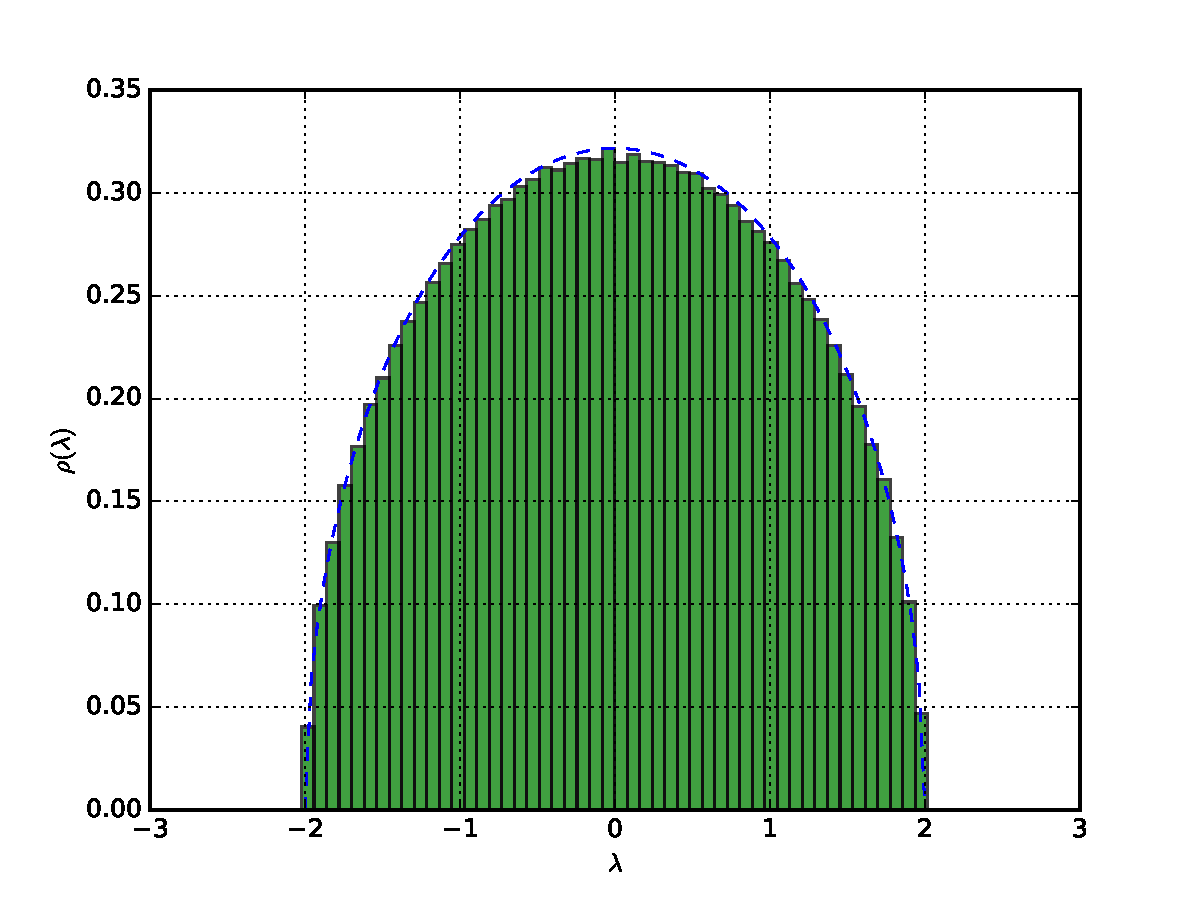
\includegraphics[width=0.75\textwidth]{../pictures/lab4_goe_eig_hist.pdf}
	\caption{Распределение нормированных собственных чисел для GOE}
	\label{fig:goe_eig}
\end{figure}
\begin{figure}[H]
	\center
	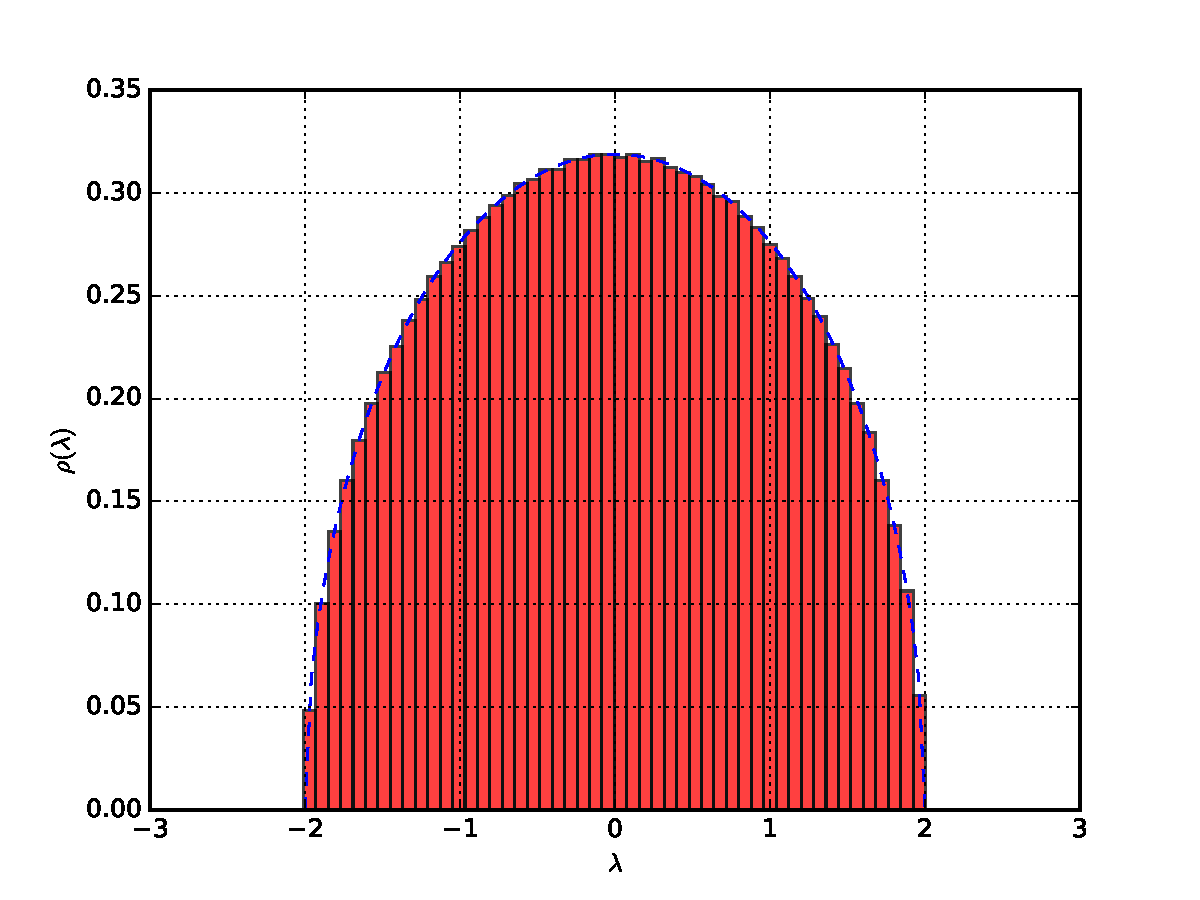
\includegraphics[width=0.75\textwidth]{../pictures/lab4_gue_eig_hist.pdf}
	\caption{Распределение нормированных собственных чисел для GUE}
	\label{fig:gue_eig}
\end{figure}

\section{Построение гистограммы расщепления уровней энергии случайных матриц}


\begin{figure}[H]
	\center
	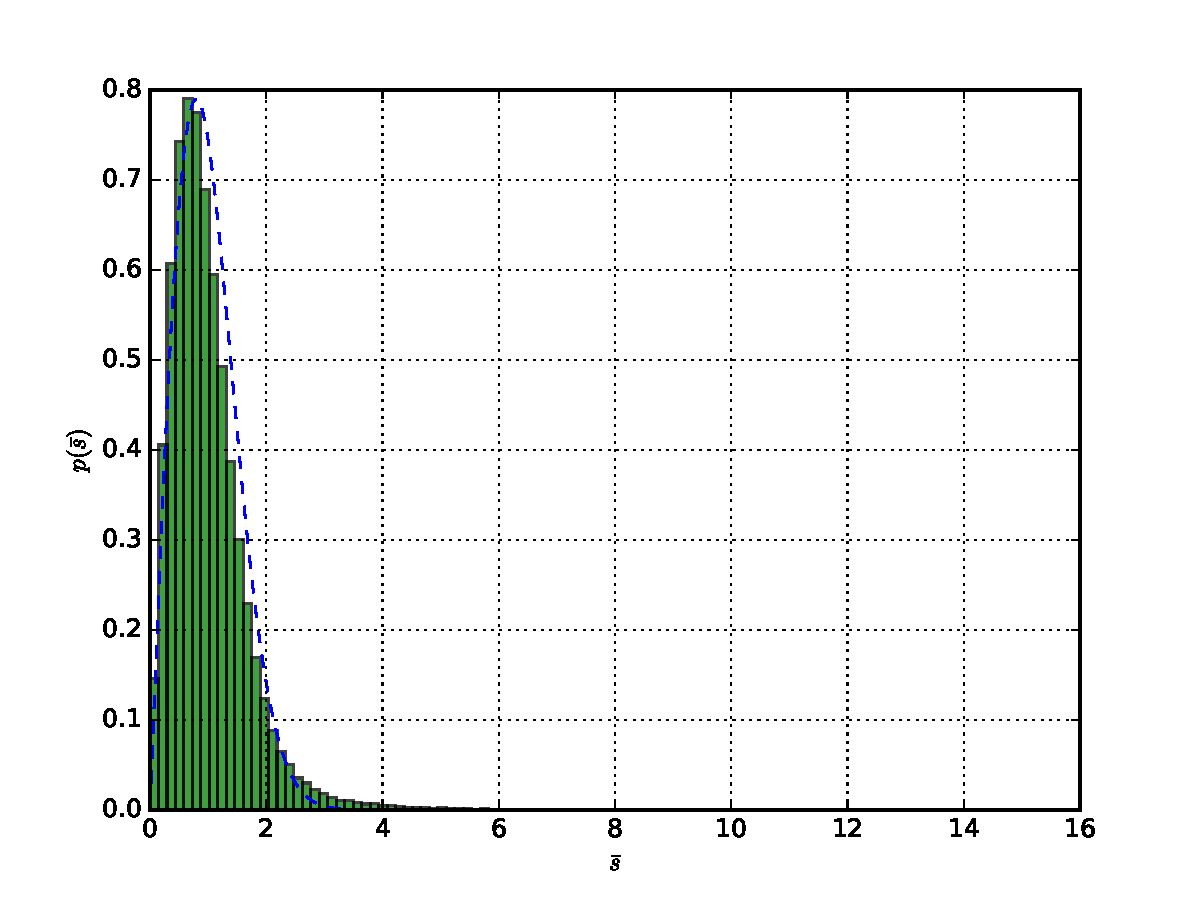
\includegraphics[width=0.75\textwidth]{../pictures/lab4_goe_spacing_hist.pdf}
	\caption{Распределение нормированных расщеплени уровней для GOE}
	\label{fig:goe_spacing}
\end{figure}

\begin{figure}[H]
	\center
	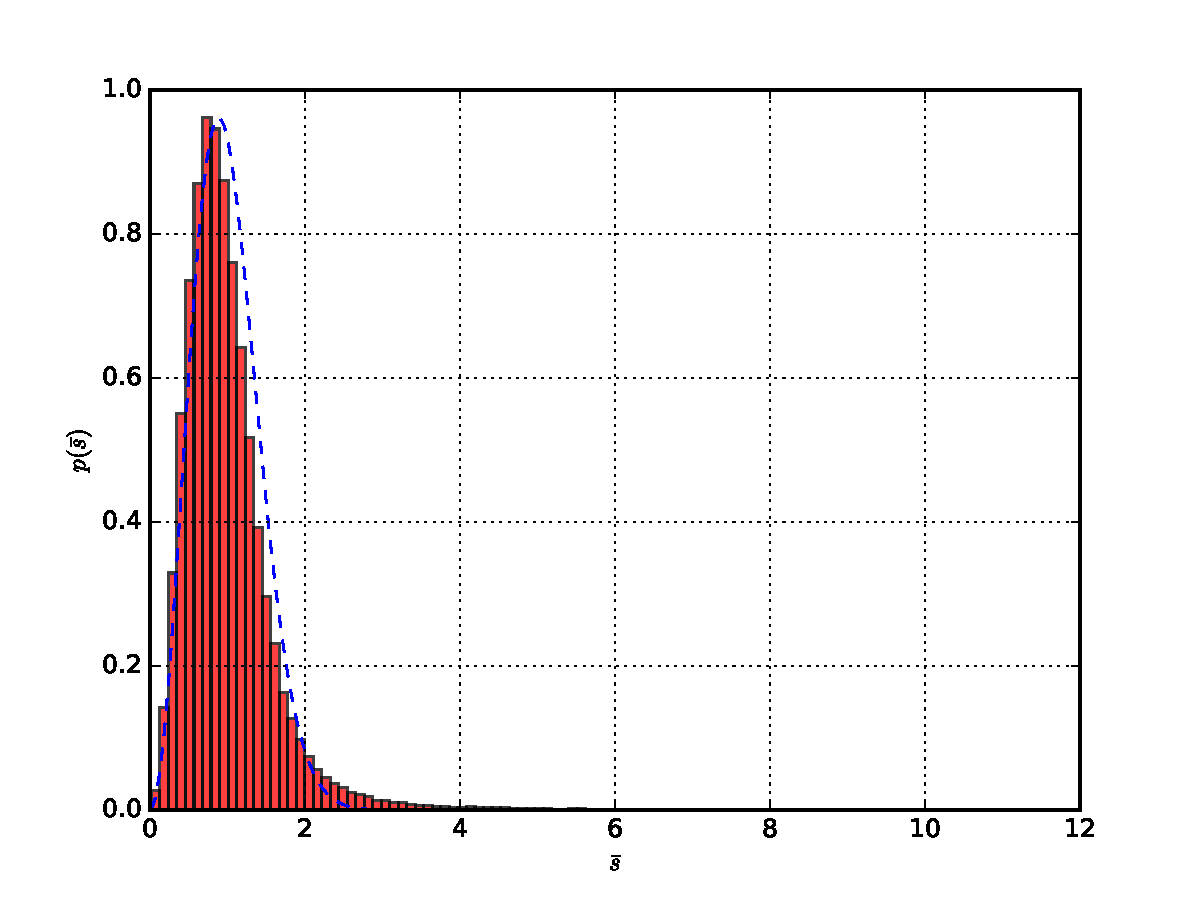
\includegraphics[width=0.75\textwidth]{../pictures/lab4_gue_spacing_hist.pdf}
	\caption{Распределение нормированных расщеплений уровней для GUE}
	\label{fig:gue_spacing}
\end{figure}


\section{Исходный код}
\lstinputlisting[language=Python, numbers=left]{../scripts/lab4.py}

\end{document}
